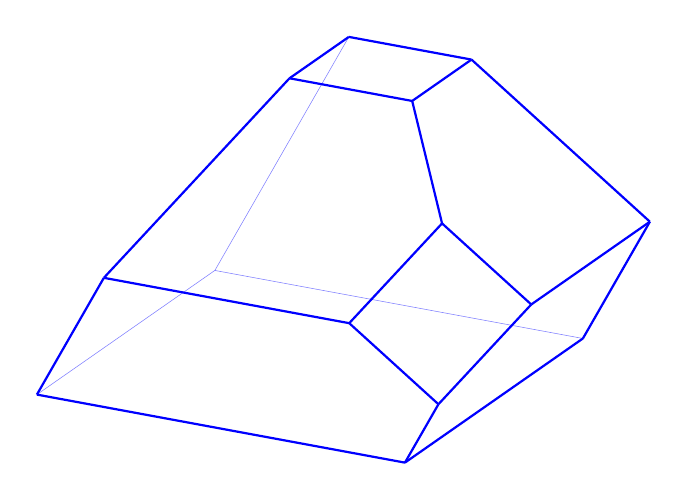
\begin{tikzpicture}%
	[x={(-0.366215cm, -0.789554cm)},
	y={(0.235950cm, -0.590693cm)},
	z={(0.900119cm, -0.166391cm)},
	scale=.5300000,
	back/.style={very thin, opacity=0.5},
	edge/.style={color=blue, thick},
	facet/.style={fill=blue,fill opacity=0},
	vertex/.style={}]
%
%
%% This TikZ-picture was produce with Sagemath version 9.5
%% with the command: ._tikz_3d_in_3d and parameters:
%% view = [-481, 324, -815]
%% angle = 141.0
%% scale = 1
%% edge_color = blue
%% facet_color = blue
%% opacity = 0.5
%% vertex_color = blue
%% axis = False

%% Coordinate of the vertices:
%%
\coordinate (1.33333, -3.77124, 3.26599) at (1.33333, -3.77124, 3.26599);
\coordinate (1.33333, -3.77124, 6.53197) at (1.33333, -3.77124, 6.53197);
\coordinate (1.33333, 1.88562, 9.79796) at (1.33333, 1.88562, 9.79796);
\coordinate (1.33333, 7.54247, -3.26599) at (1.33333, 7.54247, -3.26599);
\coordinate (1.33333, 7.54247, 6.53197) at (1.33333, 7.54247, 6.53197);
\coordinate (4.00000, -5.65685, 3.26599) at (4.00000, -5.65685, 3.26599);
\coordinate (4.00000, -5.65685, 6.53197) at (4.00000, -5.65685, 6.53197);
\coordinate (6.66667, -4.71405, 8.16497) at (6.66667, -4.71405, 8.16497);
\coordinate (6.66667, -1.88562, 9.79796) at (6.66667, -1.88562, 9.79796);
\coordinate (9.33333, -3.77124, 0.00000) at (9.33333, -3.77124, 0.00000);
\coordinate (9.33333, -3.77124, 6.53197) at (9.33333, -3.77124, 6.53197);
\coordinate (9.33333, -0.94281, 8.16497) at (9.33333, -0.94281, 8.16497);
\coordinate (9.33333, 1.88562, -3.26599) at (9.33333, 1.88562, -3.26599);
\coordinate (9.33333, 1.88562, 6.53197) at (9.33333, 1.88562, 6.53197);
%%
%%
%% Drawing edges in the back
%%
\draw[edge,back] (1.33333, -3.77124, 3.26599) -- (1.33333, 7.54247, -3.26599);
\draw[edge,back] (1.33333, 7.54247, -3.26599) -- (1.33333, 7.54247, 6.53197);
\draw[edge,back] (1.33333, 7.54247, -3.26599) -- (9.33333, 1.88562, -3.26599);
%%
%%
%% Drawing vertices in the back
%%
\node[vertex] at (1.33333, 7.54247, -3.26599)     {};
%%
%%
%% Drawing the facets
%%
\fill[facet] (9.33333, -3.77124, 6.53197) -- (6.66667, -4.71405, 8.16497) -- (4.00000, -5.65685, 6.53197) -- (4.00000, -5.65685, 3.26599) -- (9.33333, -3.77124, 0.00000) -- cycle {};
\fill[facet] (6.66667, -1.88562, 9.79796) -- (1.33333, 1.88562, 9.79796) -- (1.33333, -3.77124, 6.53197) -- (4.00000, -5.65685, 6.53197) -- (6.66667, -4.71405, 8.16497) -- cycle {};
\fill[facet] (4.00000, -5.65685, 6.53197) -- (1.33333, -3.77124, 6.53197) -- (1.33333, -3.77124, 3.26599) -- (4.00000, -5.65685, 3.26599) -- cycle {};
\fill[facet] (9.33333, -0.94281, 8.16497) -- (6.66667, -1.88562, 9.79796) -- (6.66667, -4.71405, 8.16497) -- (9.33333, -3.77124, 6.53197) -- cycle {};
\fill[facet] (9.33333, 1.88562, 6.53197) -- (1.33333, 7.54247, 6.53197) -- (1.33333, 1.88562, 9.79796) -- (6.66667, -1.88562, 9.79796) -- (9.33333, -0.94281, 8.16497) -- cycle {};
\fill[facet] (9.33333, 1.88562, 6.53197) -- (9.33333, -0.94281, 8.16497) -- (9.33333, -3.77124, 6.53197) -- (9.33333, -3.77124, 0.00000) -- (9.33333, 1.88562, -3.26599) -- cycle {};
%%
%%
%% Drawing edges in the front
%%
\draw[edge] (1.33333, -3.77124, 3.26599) -- (1.33333, -3.77124, 6.53197);
\draw[edge] (1.33333, -3.77124, 3.26599) -- (4.00000, -5.65685, 3.26599);
\draw[edge] (1.33333, -3.77124, 6.53197) -- (1.33333, 1.88562, 9.79796);
\draw[edge] (1.33333, -3.77124, 6.53197) -- (4.00000, -5.65685, 6.53197);
\draw[edge] (1.33333, 1.88562, 9.79796) -- (1.33333, 7.54247, 6.53197);
\draw[edge] (1.33333, 1.88562, 9.79796) -- (6.66667, -1.88562, 9.79796);
\draw[edge] (1.33333, 7.54247, 6.53197) -- (9.33333, 1.88562, 6.53197);
\draw[edge] (4.00000, -5.65685, 3.26599) -- (4.00000, -5.65685, 6.53197);
\draw[edge] (4.00000, -5.65685, 3.26599) -- (9.33333, -3.77124, 0.00000);
\draw[edge] (4.00000, -5.65685, 6.53197) -- (6.66667, -4.71405, 8.16497);
\draw[edge] (6.66667, -4.71405, 8.16497) -- (6.66667, -1.88562, 9.79796);
\draw[edge] (6.66667, -4.71405, 8.16497) -- (9.33333, -3.77124, 6.53197);
\draw[edge] (6.66667, -1.88562, 9.79796) -- (9.33333, -0.94281, 8.16497);
\draw[edge] (9.33333, -3.77124, 0.00000) -- (9.33333, -3.77124, 6.53197);
\draw[edge] (9.33333, -3.77124, 0.00000) -- (9.33333, 1.88562, -3.26599);
\draw[edge] (9.33333, -3.77124, 6.53197) -- (9.33333, -0.94281, 8.16497);
\draw[edge] (9.33333, -0.94281, 8.16497) -- (9.33333, 1.88562, 6.53197);
\draw[edge] (9.33333, 1.88562, -3.26599) -- (9.33333, 1.88562, 6.53197);
%%
%%
%% Drawing the vertices in the front
%%
\node[vertex] at (1.33333, -3.77124, 3.26599)     {};
\node[vertex] at (1.33333, -3.77124, 6.53197)     {};
\node[vertex] at (1.33333, 1.88562, 9.79796)     {};
\node[vertex] at (1.33333, 7.54247, 6.53197)     {};
\node[vertex] at (4.00000, -5.65685, 3.26599)     {};
\node[vertex] at (4.00000, -5.65685, 6.53197)     {};
\node[vertex] at (6.66667, -4.71405, 8.16497)     {};
\node[vertex] at (6.66667, -1.88562, 9.79796)     {};
\node[vertex] at (9.33333, -3.77124, 0.00000)     {};
\node[vertex] at (9.33333, -3.77124, 6.53197)     {};
\node[vertex] at (9.33333, -0.94281, 8.16497)     {};
\node[vertex] at (9.33333, 1.88562, -3.26599)     {};
\node[vertex] at (9.33333, 1.88562, 6.53197)     {};
%%
%%
\end{tikzpicture}